%% LyX 2.3.4.2 created this file.  For more info, see http://www.lyx.org/.
%% Do not edit unless you really know what you are doing.
\documentclass[english]{article}
\usepackage[T1]{fontenc}
\usepackage[latin9]{inputenc}
\usepackage{geometry}
\geometry{verbose,tmargin=1in,bmargin=1in,lmargin=1in,rmargin=1in}
\usepackage{color}
\usepackage{verbatim}
\usepackage{float}
\usepackage{amsmath}
\usepackage{amssymb}
\usepackage{stackrel}
\usepackage{graphicx}

\makeatletter
%%%%%%%%%%%%%%%%%%%%%%%%%%%%%% User specified LaTeX commands.
\newcommand{\RR}{\mathbb{R}^{2}}
\newcommand{\Qi}{Q_{i}}
\newcommand{\Qj}{Q_{j}}
\newcommand{\sgnDist}{b}
\newcommand{\posi}{p_{i}}
\newcommand{\pos}{p}
\newcommand{\posrel}{\tilde{p}}
\newcommand{\vel}{v}
\newcommand{\velrel}{v}
\newcommand{\pix}{p_{i,x}}
\newcommand{\piy}{p_{i,y}}
\newcommand{\veli}{v_{i}}
\newcommand{\smax}{s_{max}}
\newcommand{\vix}{v_{i,x}}
\newcommand{\viy}{v_{i,y}}
\newcommand{\ui}{u_i}
\newcommand{\uix}{u_{i,x}}
\newcommand{\uiy}{u_{i,y}}
\newcommand{\uis}{u_{i,s}}
\newcommand{\uitheta}{u_{i,\theta}}
\newcommand{\pjx}{p_{j,x}}
\newcommand{\pjy}{p_{j,y}}
\newcommand{\vjx}{v_{j,x}}
\newcommand{\vjy}{v_{j,y}}
\newcommand{\ujx}{u_{j,x}}
\newcommand{\ujy}{u_{j,y}}
\newcommand{\dx}{d_{x}}
\newcommand{\dy}{d_{y}}
\newcommand{\thetai}{\theta_{i}}
\newcommand{\si}{s_{i}}

\newcommand{\vxr}{v_{r,x}}
\newcommand{\vyr}{v_{r,y}}
\newcommand{\pxr}{p_{r,x}}
\newcommand{\pyr}{p_{r,y}}
\newcommand{\vdxr}{\dot{v}_{r,x}}
\newcommand{\vdyr}{\dot{v}_{r,y}}
\newcommand{\pdxr}{\dot{p}_{r,x}}
\newcommand{\pdyr}{\dot{p}_{r,y}}

\newcommand{\ttr}{\psi}
\newcommand{\rd}{r_d}
\newcommand{\rO}{r_0}
\newcommand{\hO}{h_0}

\newcommand{\qedwhite}{\hfill \ensuremath{\Box}}

\makeatother

\usepackage{babel}
\begin{document}

\section{Double Integrator Model}

\subsection{Problem Formulation}

We consider a group of $N$ vehicles, each of them denoted $Q_{i}$,
$i=1,\cdots,N$. Each vehicle with dynamics described by 
\begin{equation}
\dot{\posi}=\veli,\,\dot{\veli}=\ui,\quad\left\Vert \veli\right\Vert \leq\smax,\,\left\Vert \left(\uix,\uiy\right)\right\Vert \leq u_{Qmax},\label{eq:problemDynamicQ}
\end{equation}

\noindent here $\posi=\left(\pix,\piy\right),$ and $\veli=\left(\vix,\viy\right)$
are the $x$ and $y$ positions and velocities of $Q_{i}$ respectively,
and $u_{i,Q}:=\left(\uix,\uiy\right)$ is the control force applied
to this mobile agent.

We consider a vehicle safe if there is no other vehicle closer than
a predefined collision radius $c_{r}$, in other words, if 
\begin{equation}
\left\Vert \pos_{i}-\pos_{j}\right\Vert >c_{r},\qquad\text{ for any }j\neq i.\label{eq:safety}
\end{equation}

\textbf{Definition} \textbf{\emph{(r-Subcover).}} A group of agents
is an $\textbf{\ensuremath{r}-subcover}$ for a compact domain $\Omega\subseteq\RR$
if: 

\begin{enumerate} 

\item The distance between any two vehicles is at least $r$. 

\item The signed distance from any vehicle to $\Omega$ is less than
equal to $-\frac{r}{2}$. 

\end{enumerate}

\textbf{Definition} $\textbf{\textit{(r-Cover).}}$ An $r$-subcover
for $\Omega$ is an $\textbf{\ensuremath{r}-cover}$ for $\Omega$
if its size is maximal (i.e., no larger number of agents can be an
$r$-subcover for $\Omega$). 

The $r$-subcover definition is closely related to finding a way to
pack circular objects of radius $\frac{r}{2}$ inside of a container
with shape $\Omega$. Having an $r$-cover implies the container is
full and there is no room for more of such objects.

\textbf{~}

\textbf{Definition (flocking around a moving target domain) {[}based
on Ref: A simple proof of CS{]} }A group of vehicles with dynamics
\ref{eq:problemDynamicQ} has a time-asymptotic flocking around a
moving target domain following the trajectory $\pos{}_{d}\left(t\right)$,
with velocity $\vel_{d}\left(t\right)$ with states if and only if
and only if its solutions $\left\{ \posi,\veli\right\} ,\,i=1,\cdots,N$
satisfy the following two conditions:

1. The relative velocity fluctuation respect the domain go to zero
time-asymptotically (veloctiy alignement):
\[
\underset{t\rightarrow+\infty}{\lim}\stackrel[i=1]{N}{\sum}\left\Vert \veli\left(t\right)-\vel_{d}\left(t\right)\right\Vert ^{2}=0
\]

2. The position fluctuations respect the domain are uniformly bounded
in time $t$ (forming a group):
\[
\underset{0\leq t<\infty}{\sup}\stackrel[i=1]{N}{\sum}\left\Vert \posi\left(t\right)-\pos_{d}\left(t\right)\right\Vert ^{2}<\infty
\]

We are interested in the following safe domain coverage problem.

$\textbf{\textit{(Safe-domain-coverage)}}$ Consider a compact domain
$\Omega$ in the plane and $N$ vehicles each with dynamics described
by \ref{eq:problemDynamicQ}, starting from safe initial conditions.
Find the maximal $r>0$ and a control policy that leads to a stable
steady state which is an $r$-cover for $\Omega$, while satisfying
the safety condition \textbackslash eqref\{eq:safety\} at any time.

\subsection{Metodology}

\subsubsection{Coverage Controller}

We consider a group of $N$ vehicles, with unconstrained dynamics
\[
\dot{\posi}=\veli,\quad\dot{\veli}=\ui.
\]

Let $\Omega\subseteq\mathbb{R}^{2}$ be a compact domain containing
zero, and define $\Omega\left(t\right)=\Omega+\pos_{d}\left(t\right)$,
where $\pos_{d}\left(t\right)$ is the solution for the system
\[
\begin{cases}
\dot{\pos_{d}} & =\vel_{d}\\
\dot{\vel_{d}} & =0,
\end{cases}
\]

\noindent we call $\pos_{d}\left(t\right)$ the marker point of the
moving domain $\Omega\left(t\right)$.

Define $\pos_{ij}:=\pos_{i}-\pos_{j}$, and $\vel_{ij}:=\vel_{i}-\vel_{j}$
and denote by $P_{\partial\Omega\left(t\right)}\left(\pos_{i}\right)$
the closest point of $\partial\Omega\left(t\right)$ to $\pos_{i}$
(i.e., the projection of $\pos_{i}$ on $\partial\Omega\left(t\right)$).
Also, define $h_{i}:=\pos_{i}-P_{\partial\Omega\left(t\right)}\left(\pos_{i}\right)$,
and denote by $\left[\left[h_{i}\right]\right]$ the signed distance
of $\pos_{i}$ from $\partial\Omega\left(t\right)$.

The proposed control force is given by:

\begin{equation}
u_{i}=\underset{\text{Inter Vehicle}}{\underbrace{-\sum_{j\neq i}^{N}f_{I}\left(\left\Vert \pos_{ij}\right\Vert \right)\frac{\pos_{ij}}{\left\Vert \pos_{ij}\right\Vert }}}-\underset{\text{Velocity Alignment}}{\underbrace{\frac{1}{N}\sum_{j\neq i}^{N}f_{al}\left(\left\Vert \pos_{ij}\right\Vert \right)\vel_{ij}}}-\overset{\text{Navigational feedback}}{\overbrace{\underset{\text{Domain Vehicle}}{\underbrace{f_{h}\left(\left[\left[h_{i}\right]\right]\right)\frac{h_{i}}{\left[\left[h_{i}\right]\right]}}}-\underset{\text{Speed Alignment}}{\underbrace{a\left(\vel_{i}-\vel_{d}\right)}}}}\label{eq:Coverage-controller}
\end{equation}

\begin{comment}
As done in {[}ref{]} we choose $f_{al}\left(\left\Vert \pos_{ij}\right\Vert \right)=C_{al}e^{-\frac{\left\Vert \pos_{ij}\right\Vert }{l_{al}}}$,
where $C_{al}$ and $l_{al}$ are constants associated to the velocity
alignment strength and
\end{comment}

The position and velocity of the $i$ th vehicle relative to the marker
of the moving domain are given by: 
\[
\begin{cases}
\posrel_{i} & :=\pos_{i}-\pos_{d}\\
\velrel_{i} & :=\vel_{i}-\vel_{d}.
\end{cases}
\]

Note that the inter-vehicle position and velocity in this new framework
satisfy:
\begin{align*}
\posrel_{ij} & :=\posrel_{i}-\posrel_{j}=\pos_{i}-\pos_{d}-\left(\pos_{j}-\pos_{d}\right)=\pos_{ij},\\
\velrel_{ij} & :=\velrel_{i}-\velrel_{j}=\vel_{i}-\vel_{d}-\left(\vel_{j}-\vel_{d}\right)=\vel_{ij},
\end{align*}

\noindent it means the relative positions are invariant to the change
of coordinates. Moreover, the vehicle domain distance satisfies $h_{i}=\pos_{i}-P_{\partial\Omega\left(t\right)}\left(\pos_{i}\right)=\left(\pos_{i}-\pos_{d}\right)-P_{\partial\Omega\left(t\right)-\pos_{d}}\left(\pos_{i}-\pos_{d}\right)=\posrel_{i}-P_{\partial\Omega\left(0\right)}\left(\posrel_{i}\right)$.
This allow us to rewrite (\ref{eq:Coverage-controller}) as
\begin{equation}
u_{i}=-\sum_{j\neq i}^{N}f_{I}\left(\left\Vert \posrel_{ij}\right\Vert \right)\frac{\posrel_{ij}}{\left\Vert \posrel_{ij}\right\Vert }-\frac{1}{N}\sum_{j\neq i}^{N}f_{al}\left(\left\Vert \posrel_{ij}\right\Vert \right)\velrel_{ij}-f_{h}\left(\left[\left[h_{i}\right]\right]\right)\frac{h_{i}}{\left[\left[h_{i}\right]\right]}-a\velrel_{i}\label{eq:Coverage-controller-rel}
\end{equation}

Let us consider the potential 
\[
V_{h}\left(\posrel_{i}\right)=\int_{-\frac{r_{d}}{2}}^{\left[\left[\posrel_{i}-P_{\partial\Omega\left(0\right)}\left(\posrel_{i}\right)\right]\right]}f_{h}\left(s\right)ds
\]

\noindent which satisfies
\[
\nabla_{\posrel_{i}}V_{h}\left(\posrel_{i}\right)=f_{h}\left(\left[\left[\posrel_{i}-P_{\partial\Omega\left(0\right)}\left(\posrel_{i}\right)\right]\right]\right)\nabla_{\posrel_{i}}\left(\left[\left[\posrel_{i}-P_{\partial\Omega\left(0\right)}\left(\posrel_{i}\right)\right]\right]\right)=f_{h}\left(\left[\left[h_{i}\right]\right]\right)\frac{h_{i}}{\left[\left[h_{i}\right]\right]}
\]

\noindent where we have used the identity $\nabla_{\posrel_{i}}\left(\left[\left[\posrel_{i}-P_{\partial\Omega\left(0\right)}\left(\posrel_{i}\right)\right]\right]\right)=\frac{\posrel_{i}-P_{\partial\Omega\left(0\right)}\left(\posrel_{i}\right)}{\left[\left[\posrel_{i}-P_{\partial\Omega\left(0\right)}\left(\posrel_{i}\right)\right]\right]}$.

Similarly, it can be shown that the inter-vehicle force is the negative
gradient of the potential 
\[
V_{I}\left(\posrel_{ij}\right)=\int_{r_{d}}^{\left\Vert \posrel_{ij}\right\Vert }f_{I}\left(s\right)ds,
\]

\noindent to finally get:
\begin{equation}
u_{i}=\underset{\text{Inter Vehicle}}{\underbrace{-\sum_{j\neq i}^{N}\nabla_{\posrel_{i}}V_{I}\left(\posrel_{ij}\right)}}-\underset{\text{Velocity Alignment}}{\underbrace{\frac{1}{N}\sum_{j\neq i}^{N}f_{al}\left(\left\Vert \posrel_{ij}\right\Vert \right)\velrel_{ij}}}-\overset{\text{Navigational feedback}}{\overbrace{\underset{\text{Domain Vehicle}}{\underbrace{\nabla_{\posrel_{i}}V_{h}\left(\posrel_{i}\right)}}-\underset{\text{Speed Alignment}}{\underbrace{a\velrel_{i}}}}}\label{eq:Coverage-controller-rel-1}
\end{equation}

\noindent Consider the candidate for Lyapunov function consisting
in kinetic plus (artificial) potential energy:
\[
\Phi=\frac{1}{2}\underset{i=1}{\overset{N}{\sum}}\Bigl(\dot{\posrel_{i}}\cdot\dot{\posrel_{i}}+\underset{j\neq i}{\overset{N}{\sum}}V_{I}\left(\posrel_{ij}\right)+V_{h}\left(\posrel_{i}\right)\Bigr).
\]

\noindent Note that each term in $\Phi$ is non-negative, and $\Phi$
reaches its absolute minimum value when the vehicles are totally stopped. 

The derivative of $\Phi$ with respect to time can be calculated as:
\begin{align*}
\dot{\Phi} & =\underset{i=1}{\overset{N}{\sum}}\dot{\posrel_{i}}\cdot\Bigl(u_{i}+\underset{j\neq i}{\overset{N}{\sum}}\nabla_{\posrel_{i}}V_{I}\left(\posrel_{ij}\right)+\nabla_{\posrel_{i}}V_{h}\left(\posrel_{i}\right)\Bigr)\\
 & =\underset{i=1}{\overset{N}{\sum}}\dot{\posrel_{i}}\cdot\left(-\frac{1}{N}\sum_{j\neq i}^{N}f_{al}\left(\left\Vert \posrel_{ij}\right\Vert \right)\velrel_{ij}-a\velrel_{i}\right)
\end{align*}

\noindent For the (extra) alignment term, write 
\[
\underset{i=1}{\overset{N}{\sum}}\velrel_{i}\cdot\underset{j\neq i}{\overset{N}{\sum}}f_{al}\left(\left\Vert \posrel_{ij}\right\Vert \right)\left(\velrel_{i}-\velrel_{j}\right)=\frac{1}{2}\underset{i=1}{\overset{N}{\sum}}\velrel_{i}\cdot\underset{j\neq i}{\overset{N}{\sum}}f_{al}\left(\left\Vert \posrel_{ij}\right\Vert \right)\left(\velrel_{i}-\velrel_{j}\right)+\frac{1}{2}\underset{j=1}{\overset{N}{\sum}}\velrel_{j}\cdot\underset{i\neq j}{\overset{N}{\sum}}f_{al}\left(\left\Vert \posrel_{ij}\right\Vert \right)\left(\velrel_{j}-\velrel_{i}\right),
\]

\noindent where in the second term in the right-hand-side we simply
rename $i\leftrightarrow j$ as indices of summation. From there,
use that $\|\posrel_{ij}\|=\|\posrel_{ji}\|$ to get:
\[
\underset{i=1}{\overset{N}{\sum}}\velrel_{i}\cdot\underset{j\neq i}{\overset{N}{\sum}}f_{al}\left(\left\Vert \posrel_{ij}\right\Vert \right)\left(\velrel_{i}-\velrel_{j}\right)=\frac{1}{2}\underset{i=1}{\overset{N}{\sum}}\underset{j\neq i}{\overset{N}{\sum}}f_{al}\left(\left\Vert \posrel_{ij}\right\Vert \right)\|\velrel_{i}-\velrel_{j}\|^{2}.
\]

\noindent With the minus sign in front this gives a negative-definite
term. Conclude that $\dot{\Phi}$ is negative semidefinite and equal
to zero if and only if $\dot{\posrel_{i}}=0$ for all $i$ (i.e.,
all vehicles are at equilibrium in the relative framework). 

~

\textbf{Theorem} Consider a group of $N$ vehicles with dynamics defined
by \ref{eq:problemDynamicQ}, and the control law given by \ref{eq:Coverage-controller}.
Let the equilibrium of interest be of the form $\dot{\posrel_{i}}=0$,
$\left\Vert \posrel_{ij}\right\Vert \geq r_{d}$ and $\left[\left[h_{i}\right]\right]\leq-\frac{r_{d}}{2}$
for $i,j=1,\cdots,N$ (see Definitions \textbackslash ref\{defn:subcover\}
and \textbackslash ref\{defn:cover\}), and assume that this equilibrium
configuration is isolated. Also assume that there is a neighborhood
about the equilibrium in which the control law remains smooth. Then,
the following statements hold: 
\begin{enumerate}
\item The group of agents has a time-asymptotic flocking around a moving
target $\Omega\left(t\right)$. 
\item Almost every solution of the relative dynamical system (to be defined)
asymptotically converges to an equilibrium point $\left(\posrel^{*},0\right)$
where $\posrel^{\ast}$ is a local minima of $V_{I}\left(\posrel\right)+V_{h}\left(\posrel\right)$. 
\item Assume the initial structural energy of the particle system is less
than $\left(k+1\right)c^{*}$ with $c^{\ast}=V_{I}\left(0\right)$
and $k\in\mathbb{Z^{+}}$. Then, at most $k$ distinct pairs of vehicles
could possibly collide ($k=0$ guarantees a collision-free motion).
\textcolor{blue}{(I have not checked this stronger result yet).}
\end{enumerate}
\textbf{proof. }To be done.

\qedwhite

It is clear that thresholding the force the theoretical guarantees
may not necessary hold anymore, however, when close to the desired
operation point the coverage input forces are small enough to not
be thresholded and it is feasible for the controller apply the required
coverage force, implying the theoretical results are locally valid.

\subsubsection*{Choosing the Adequate Cucker Smale Parameters}

We assume as premise that the major velocity alignment effects should
be for those vehicles within an $r_{d}$ radius neighborhood. It seems
wide enough to guarantee flocking behavior without causing group inertia
that may slow down the domain coverage aim. In order to so, we impose
a tenth decay on the alignment strength every \textbf{$r_{d}$}, i.e.
$l_{al}=-\frac{r_{d}}{\ln\left(0.1\right)}$.

\subsubsection{Collision Avoidance via Analytic HJI PDE Solution}

\textcolor{blue}{(I think we should call the result from the paper
for the analytical solution of the HJ eq instead of redoing it here).}

\section{Fixed-wing model}

Similarly as before we consider a group of $N$ vehicles, each of
them denoted $W_{i}$, $i=1,\cdots,N$, but this time with dynamics
described by 
\begin{equation}
\dot{\pos_{i}}=\si\left(\cos\left(\thetai\right),\sin\left(\thetai\right)\right),\,\dot{\thetai}=u_{i,\theta},\,\dot{\si}=\uis,\quad\left|\si\right|\leq\smax\,\left|\uitheta\right|\leq u_{\theta\,max},\,\left|\uis\right|\leq u_{s\,max}\label{eq:problemDynamicW}
\end{equation}

\noindent here $\posi=\left(\pix,\piy\right),$ and $\veli=\left(\vix,\viy\right)$
are the $x$ and $y$ positions and velocities respectively, $\thetai$
is the heading angle and $\si$ the speed of the vehicle $W_{i}$.
Additionally, the acceleration is $u_{i,W}:=\left(\uitheta,\uis\right)$.

\subsection{Thresholding Coverage Control Force}

As we assume constrained input forces, we to need modify the proposed
coverage control force when necessary. For the double integrator model
the given coverage control force $u=\left(u_{x},u_{y}\right)$ is
projected onto the set of admissible forces using the mapping,
\[
\hat{u}=\begin{cases}
u & \text{if }\left\Vert u\right\Vert \leq u_{max},\\
u_{max}\frac{u}{\left\Vert u\right\Vert } & \text{otherwise.}
\end{cases}
\]

On the other hand, in order to get the appropriate Dubins car control
force we use the relation
\begin{equation}
\frac{d}{dt}\left(\begin{array}{c}
v_{x}\\
v_{y}
\end{array}\right)=R\left(v,\theta\right)\left(\begin{array}{c}
u_{\theta}\\
u_{v}
\end{array}\right);\,R\left(v,\theta\right):=\left(\begin{array}{cc}
v\sin\left(\theta\right) & \cos\left(\theta\right)\\
v\cos\left(\theta\right) & -\sin\left(\theta\right)
\end{array}\right),\label{eq:DubinsToRec}
\end{equation}

\noindent which allow us to represent the set of admissible forces
from the $xy$ perspective as the region 
\[
S=\left\{ R\left(v,\theta\right)\left(\begin{array}{c}
u_{\theta}\\
u_{v}
\end{array}\right):\left(\begin{array}{c}
u_{\theta}\\
u_{v}
\end{array}\right)\in\left[-u_{\theta max},u_{\theta max}\right]\times\left[-u_{vmax},u_{vmax}\right]\right\} 
\]

we set $\left(\begin{array}{c}
\hat{u}_{x}\\
\hat{u}_{y}
\end{array}\right)=\sup\left\{ t\in\mathbb{R}:t\left(\begin{array}{c}
u_{x}\\
u_{y}
\end{array}\right)\in S\right\} \left(\begin{array}{c}
u_{x}\\
u_{y}
\end{array}\right)$, see Fig. \ref{fig:Thresholding-Dubins-car}. Finally, we get the
associated Dubins car input force by inverting (\ref{eq:DubinsToRec})
as $\left(\begin{array}{c}
\hat{u}_{\theta}\\
\hat{u}_{v}
\end{array}\right)=R^{-1}\left(v,\theta\right)\left(\begin{array}{c}
\hat{u}_{x}\\
\hat{u}_{y}
\end{array}\right)$.

\begin{figure}[H]
\begin{centering}
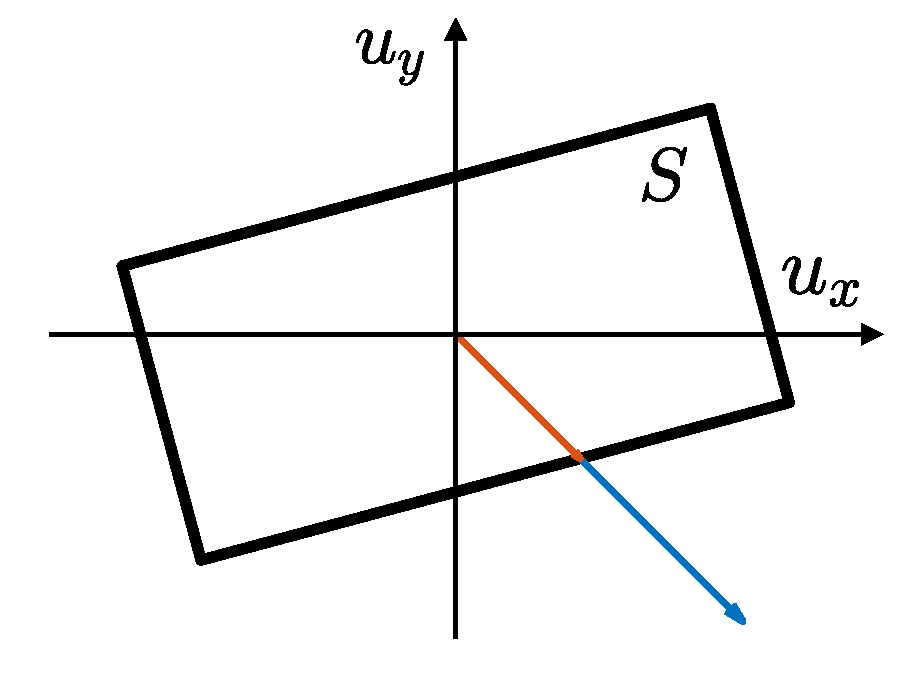
\includegraphics[width=0.4\columnwidth]{../../self-propelling/notes/forceThreshold}
\par\end{centering}
\caption{\label{fig:Thresholding-Dubins-car}Thresholding Dubins car force
in rectangular coordinates.}
\end{figure}


\subsection{Collision avoidance}

\begin{align*}
\left(\begin{array}{c}
x_{1}\\
x_{2}
\end{array}\right) & =\left(\begin{array}{cc}
\cos\left(\theta_{1}\right) & \sin\left(\theta_{1}\right)\\
-\sin\left(\theta_{1}\right) & \cos\left(\theta_{1}\right)
\end{array}\right)\left(\begin{array}{c}
p_{x,2}-p_{x,1}\\
p_{y,2}-p_{y,1}
\end{array}\right)=\left(\begin{array}{c}
\cos\left(\theta_{1}\right)\left(p_{x,2}-p_{x,1}\right)+\sin\left(\theta_{1}\right)\left(p_{y,2}-p_{y,1}\right)\\
-\sin\left(\theta_{1}\right)\left(p_{x,2}-p_{x,1}\right)+\cos\left(\theta_{1}\right)\left(p_{y,2}-p_{y,1}\right)
\end{array}\right)
\end{align*}

\begin{align*}
\left(\begin{array}{c}
\dot{x_{1}}\\
\dot{x_{2}}
\end{array}\right) & =\left(\begin{array}{c}
-\dot{\theta_{1}}\sin\left(\theta_{1}\right)\left(p_{x,2}-p_{x,1}\right)+\cos\left(\theta_{1}\right)\left(\dot{p}_{x,2}-\dot{p}_{x,1}\right)+\dot{\theta_{1}}\cos\left(\theta_{1}\right)\left(p_{y,2}-p_{y,1}\right)+\sin\left(\theta_{1}\right)\left(\dot{p}_{y,2}-\dot{p}_{y,1}\right)\\
-\dot{\theta_{1}}\cos\left(\theta_{1}\right)\left(p_{x,2}-p_{x,1}\right)-\sin\left(\theta_{1}\right)\left(\dot{p}_{x,2}-\dot{p}_{x,1}\right)-\dot{\theta_{1}}\sin\left(\theta_{1}\right)\left(p_{y,2}-p_{y,1}\right)+\cos\left(\theta_{1}\right)\left(\dot{p}_{y,2}-\dot{p}_{y,1}\right)
\end{array}\right)\\
 & =\left(\begin{array}{c}
\cos\left(\theta_{1}\right)\left(v_{2}\cos\left(\theta_{2}\right)-v_{1}\cos\left(\theta_{1}\right)\right)+\sin\left(\theta_{1}\right)\left(v_{2}\sin\left(\theta_{2}\right)-v_{1}\sin\left(\theta_{1}\right)\right)+\dot{\theta_{1}}x_{2}\\
-\sin\left(\theta_{1}\right)\left(v_{2}\cos\left(\theta_{2}\right)-v_{1}\cos\left(\theta_{1}\right)\right)+\cos\left(\theta_{1}\right)\left(v_{2}\sin\left(\theta_{2}\right)-v_{1}\sin\left(\theta_{1}\right)\right)-\dot{\theta_{1}}x_{1}
\end{array}\right)\\
 & =\left(\begin{array}{c}
v_{2}\cos\left(\theta_{2}-\theta_{1}\right)-v_{1}+\dot{\theta_{1}}x_{2}\\
v_{2}\sin\left(\theta_{2}-\theta_{1}\right)-\dot{\theta_{1}}x_{1}
\end{array}\right)
\end{align*}

\[
\left(\begin{array}{c}
x_{1}\\
x_{2}\\
x_{3}\\
x_{4}\\
x_{5}
\end{array}\right)=\left(\begin{array}{c}
\cos\left(\theta_{1}\right)\left(p_{x,2}-p_{x,1}\right)+\sin\left(\theta_{1}\right)\left(p_{y,2}-p_{y,1}\right)\\
-\sin\left(\theta_{1}\right)\left(p_{x,2}-p_{x,1}\right)+\cos\left(\theta_{1}\right)\left(p_{y,2}-p_{y,1}\right)\\
\theta_{2}-\theta_{1}\\
v_{1}\\
v_{2}
\end{array}\right)
\]

\[
\dot{\left(\begin{array}{c}
x_{1}\\
x_{2}\\
x_{3}\\
x_{4}\\
x_{5}
\end{array}\right)}=\left(\begin{array}{c}
x_{5}\cos\left(x_{3}\right)-x_{4}+u_{\theta}x_{2}\\
x_{5}\sin\left(x_{3}\right)-u_{\theta}x_{1}\\
d_{\theta}-u_{\theta}\\
u_{v}\\
d_{v}
\end{array}\right)
\]

Optimal controller: $u_{\theta}^{*}=\text{sgn}\left(\frac{\partial V}{\partial x_{1}}x_{2}-\frac{\partial V}{\partial x_{2}}x_{1}-\frac{\partial V}{\partial x_{3}}\right)u_{\theta max}$,
$u_{v}^{*}=\text{sgn}\left(\frac{\partial V}{\partial x_{4}}\right)u_{vmax}$

Optimal disturbance: $d_{\theta}^{*}=-\text{sgn}\left(\frac{\partial V}{\partial x_{3}}\right)d_{\theta max}$,
$d_{v}^{*}=-\text{sgn}\left(\frac{\partial V}{\partial x_{5}}\right)d_{vmax}$
\end{document}
